% Preambulo do manuscrito. Compilar de dentro de paper/:
%   tectonic -X compile manuscript.tex --outdir ../build
\documentclass[11pt]{article}

\usepackage[margin=1in]{geometry}
\usepackage[T1]{fontenc}
\usepackage[utf8]{inputenc}
\usepackage{lmodern}

\usepackage{setspace}
\usepackage{lineno}
\usepackage{booktabs}
\usepackage{multirow}
\usepackage{graphicx}
\usepackage{pgfplots}      % figura como codigo: entra por \input, nao como anexo
\pgfplotsset{compat=1.18}
\usepackage{xurl}
\usepackage{xcolor}
\usepackage{caption}
\usepackage{amsmath}
% Tres legendas dependem daqui, nao uma: fig4_janela e revisao_fig_enriched_janela
% usam \blacksquare, e revisao_fig_temp_diffcal usa \square. Sem amssymb o documento
% inteiro para de compilar, ainda que a figura isolada compile: o preambulo que o
% gerador monta para compilar cada figura sozinha ja o carrega.
% Os tres simbolos saem dos geradores (build_paper_assets.py e
% revisao/build_revisao_figs2.py), entao sobrevivem a qualquer regeneracao. Quem
% cobra essa correspondencia e tests/test_latex_saudavel.py.
\usepackage{amssymb}
\usepackage[numbers,sort&compress]{natbib}

\captionsetup{font=small,labelfont=bf}
\graphicspath{{figures/}}

% Paleta das figuras, definida uma vez aqui em vez de repetida em cada uma.
% Okabe-Ito (Wong, 2011): distinguivel sob deuteranopia, protanopia e tritanopia, e
% legivel em impressao P&B.
%
% Estes HEX tem de ser os mesmos de COR em scripts/build_paper_assets.py, que e a
% paleta usada ao rasterizar as figuras em PNG. Eles ficaram tres semanas divergentes:
% o gerador migrou para Okabe-Ito e o preambulo continuou na paleta antiga do seaborn,
% entao a MESMA figura saia com cores diferentes no PDF e no .docx, e a do PDF era a
% que confunde vermelho com verde. Quem cobra a igualdade agora e
% tests/test_latex_saudavel.py, porque o comentario sozinho ja falhou nisso.
\definecolor{cprophet}{HTML}{0072B2}
\definecolor{csarima}{HTML}{D55E00}
\definecolor{ctimesfm}{HTML}{009E73}
\definecolor{cxgboost}{HTML}{E69F00}
\definecolor{ccatboost}{HTML}{CC79A7}
% Papel, nao modelo: reservada para a covariavel de temperatura.
\definecolor{ctemp}{HTML}{56B4E9}

% Marcador de dado ainda indisponivel. Sai vermelho e em negrito de proposito:
% e para ser impossivel submeter sem ver.
\newcommand{\missing}[1]{\textcolor{red}{\textbf{[MISSING: #1]}}}

% Marcador de decisao ainda nao tomada, ao lado do texto que ela afeta. Mesmo
% vermelho do \missing e pelo mesmo motivo: o trecho entre colchetes nao pode
% escapar para a submissao sem alguem ter olhado.
\newcommand{\aberto}[1]{\textcolor{red}{\textbf{[OPEN: #1]}}}

\setstretch{1.5}
\linenumbers


\title{\vspace{-2em}\large\bfseries Training history and model choice in forecasting monthly
cardiovascular mortality in S\~ao Paulo, Brazil: foundation, classical and boosting models
compared with paired uncertainty}

\ifdefined\BLIND
\author{}
\else
\author{Fabiano Novaes Barcellos Filho\thanks{Faculdade de Sa\'ude P\'ublica, Universidade de
S\~ao Paulo, S\~ao Paulo, Brazil. Corresponding author.} \and
Isabela Venancio da Silva\footnotemark[1] \and
Victor Hugo Ovani Marchetti\footnotemark[1] \and
Alexandre Chiavegatto Filho\footnotemark[1]}
\fi

\date{}

\begin{document}
\maketitle

\noindent\textbf{Running title:} Forecasting cardiovascular mortality in S\~ao Paulo \\
\textbf{Keywords:} cardiovascular mortality; time series forecasting; foundation models;
prediction intervals; health surveillance; Brazil

\vspace{1em}
\hrule
\vspace{1em}

\section*{Abstract}

Health services that plan for the winter rise in cardiovascular deaths need monthly
forecasts, and a growing number of studies propose pre-trained foundation models for this
task. We compared SARIMA, Prophet, the TimesFM foundation model, XGBoost and CatBoost on the
monthly count of cardiovascular deaths in S\~ao Paulo state, Brazil, from 2010 to 2023
(1{,}217{,}427 deaths), using 103 rolling origin windows with a 6-month horizon and paired
block bootstrap intervals. Prophet, SARIMA and TimesFM reached sMAPE between 4.70\% and
4.83\%, and none of the three pairwise differences was distinguishable from zero. Both
boosting models were worse than all three and did not improve on repeating the same month
of the previous year. On identical target months, nine additional years of training reduced
error by 1.23 to 1.71 percentage points, about ten times the spread among the three leading
models. When training was limited to the last five years, SARIMA and Prophet lost accuracy
and TimesFM did not. The native 95\% intervals of SARIMA and Prophet covered 84.5\% and
77.2\% of observations. For a single indicator with a long record, the choice among these
models matters less than the length of the series and the calibration of the intervals.

\vspace{1em}
\hrule

\section{Introduction}

Cardiovascular diseases cause about 17.9 million deaths a year worldwide \citep{roth2020}
and have been the leading cause of death in Brazil since the 1960s, around 30\% of all
deaths in recent decades \citep{oliveira2020, brant2017}. Age-standardised rates have fallen
since the 1990s \citep{ribeiro2016}, but population growth and ageing keep the absolute
number rising \citep{brant2025}: in S\~ao Paulo, the most populous state, annual
cardiovascular deaths went from 79{,}933 in 2010 to 95{,}538 in 2023. The burden is also
seasonal. Mortality from myocardial infarction in the city of S\~ao Paulo rises in winter
\citep{sharovsky2002}, and among six Brazilian micro-regions studied by \citet{ferreira2019},
S\~ao Paulo had the largest number of deaths from myocardial infarction attributed to cold. Coronary and stroke beds, emergency staff
and drug supply have to be arranged before that peak, which is the use a monthly forecast
of deaths serves. \aberto{one or two sentences from the authors on how forecasts of this
series are, or could be, used in state planning}

Forecasts of cardiovascular mortality in Brazil have addressed long-range trends:
\citet{siqueira2020}, for example, projected mortality from myocardial
infarction, stroke and heart failure to 2030 in five-year intervals. Monthly forecasting
over a horizon of a few months is a different problem, and the methods on offer for it have
changed. Seasonal ARIMA \citep{box2015} and Prophet \citep{taylor2018} estimate a model from
the target series itself. Foundation models such as TimesFM \citep{das2024} and Chronos
\citep{ansari2024} are pre-trained on large collections of series and forecast a new one
without task-specific training, and health-specific variants are appearing \citep{li2025}.
Gradient boosting, which dominated the M5 competition \citep{makridakis2022}, is the usual choice
when forecasting is posed as a tabular problem.

How these families compare on one health series is less settled than benchmark leaderboards
suggest. Foundation models are evaluated on archives of thousands of series
\citep{godahewa2021, aksu2024}, and an average rank across an archive does not say which
model to use for a particular indicator. Backtesting a single series produces forecasts from
overlapping windows that share training data, so aggregate errors carry wide intervals, and
differences of a few tenths of a percentage point are easily within them
\citep{hewamalage2023}. The question for a surveillance team is therefore twofold: whether
any of these models is measurably better on its own series, and what else affects accuracy
that the team can control.

We addressed both on the monthly series of cardiovascular deaths in S\~ao Paulo state from
2010 to 2023. We compared five models and three naive references on identical rolling
origin windows, with paired intervals for every comparison. We then varied the amount of
training history while holding the test months fixed, measured the coverage of the
prediction intervals that two of the models produce, and tested monthly temperature as a
covariate.

\section{Methods}\label{sec:metodos}

\subsection{Data}

We used individual death records from the Mortality Information System (SIM) of the
Brazilian Ministry of Health, distributed by DataSUS \citep{datasus}, for residents of S\~ao
Paulo state from January 2010 to December 2023. Of 4{,}317{,}224 records, 1{,}217{,}427 had
an underlying cause in ICD-10 chapter IX, diseases of the circulatory system (I00--I99)
\citep{icd10}. Aggregated by month of death, they form a series of 168 points with a mean of
7{,}247 deaths (median 7{,}177), a minimum of 5{,}811 in February 2011 and a maximum of
9{,}582 in January 2022 (Figure~\ref{fig:serie}). Death registration in the state is close
to complete, estimated at 99.9\% in 2016 by record linkage \citep{costa2020}. We did not
redistribute ill-defined causes (garbage codes), so counts are not directly comparable with
Global Burden of Disease estimates.

\begin{figure}[htbp]
\centering
% gerado por scripts/build_paper_assets.py -- nao editar a mao
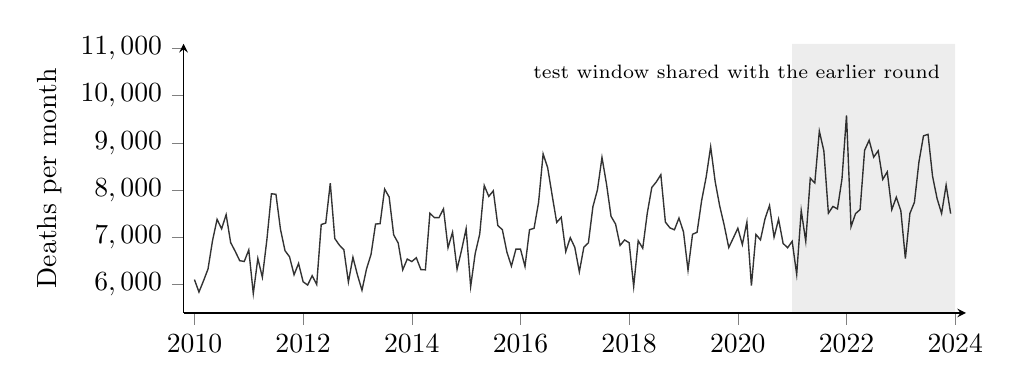
\begin{tikzpicture}
\begin{axis}[
  width=0.95\textwidth, height=5.0cm,
  xlabel={}, ylabel={Deaths per month},
  xmin=2009.8, xmax=2024.2, ymin=5400, ymax=11100,
  xtick={2010,2012,2014,2016,2018,2020,2022,2024},
  xticklabel style={/pgf/number format/1000 sep=},
  % sem isto o pgfplots troca o eixo por \cdot 10^4, que e ilegivel aqui
  scaled y ticks=false,
  ytick={6000,7000,8000,9000,10000,11000},
  yticklabel style={/pgf/number format/fixed, /pgf/number format/1000 sep={,}},
  axis lines=left, tick align=outside, tick pos=left,
  every axis plot/.append style={line width=0.5pt},
]
\addplot[draw=black!80, mark=none] coordinates {(2010.0000,6107) (2010.0833,5843) (2010.1667,6079) (2010.2500,6332) (2010.3333,6934) (2010.4167,7382) (2010.5000,7182) (2010.5833,7481) (2010.6667,6890) (2010.7500,6706) (2010.8333,6507) (2010.9167,6490) (2011.0000,6735) (2011.0833,5811) (2011.1667,6554) (2011.2500,6156) (2011.3333,6952) (2011.4167,7924) (2011.5000,7913) (2011.5833,7172) (2011.6667,6719) (2011.7500,6590) (2011.8333,6208) (2011.9167,6448) (2012.0000,6060) (2012.0833,5991) (2012.1667,6189) (2012.2500,6004) (2012.3333,7272) (2012.4167,7304) (2012.5000,8148) (2012.5833,6976) (2012.6667,6837) (2012.7500,6738) (2012.8333,6054) (2012.9167,6579) (2013.0000,6205) (2013.0833,5881) (2013.1667,6331) (2013.2500,6640) (2013.3333,7283) (2013.4167,7291) (2013.5000,8023) (2013.5833,7855) (2013.6667,7054) (2013.7500,6880) (2013.8333,6314) (2013.9167,6542) (2014.0000,6488) (2014.0833,6569) (2014.1667,6318) (2014.2500,6313) (2014.3333,7512) (2014.4167,7418) (2014.5000,7417) (2014.5833,7605) (2014.6667,6781) (2014.7500,7110) (2014.8333,6327) (2014.9167,6734) (2015.0000,7184) (2015.0833,5958) (2015.1667,6658) (2015.2500,7069) (2015.3333,8099) (2015.4167,7868) (2015.5000,7986) (2015.5833,7251) (2015.6667,7163) (2015.7500,6690) (2015.8333,6392) (2015.9167,6753) (2016.0000,6753) (2016.0833,6385) (2016.1667,7164) (2016.2500,7192) (2016.3333,7743) (2016.4167,8767) (2016.5000,8479) (2016.5833,7890) (2016.6667,7317) (2016.7500,7426) (2016.8333,6700) (2016.9167,6994) (2017.0000,6788) (2017.0833,6271) (2017.1667,6794) (2017.2500,6884) (2017.3333,7651) (2017.4167,8009) (2017.5000,8694) (2017.5833,8130) (2017.6667,7446) (2017.7500,7282) (2017.8333,6830) (2017.9167,6946) (2018.0000,6886) (2018.0833,5960) (2018.1667,6930) (2018.2500,6769) (2018.3333,7511) (2018.4167,8057) (2018.5000,8175) (2018.5833,8328) (2018.6667,7325) (2018.7500,7202) (2018.8333,7161) (2018.9167,7409) (2019.0000,7117) (2019.0833,6307) (2019.1667,7067) (2019.2500,7108) (2019.3333,7776) (2019.4167,8274) (2019.5000,8919) (2019.5833,8180) (2019.6667,7664) (2019.7500,7254) (2019.8333,6785) (2019.9167,6987) (2020.0000,7194) (2020.0833,6848) (2020.1667,7324) (2020.2500,5978) (2020.3333,7062) (2020.4167,6948) (2020.5000,7392) (2020.5833,7678) (2020.6667,7005) (2020.7500,7385) (2020.8333,6872) (2020.9167,6781) (2021.0000,6917) (2021.0833,6217) (2021.1667,7569) (2021.2500,6917) (2021.3333,8253) (2021.4167,8153) (2021.5000,9251) (2021.5833,8830) (2021.6667,7512) (2021.7500,7656) (2021.8333,7603) (2021.9167,8237) (2022.0000,9582) (2022.0833,7227) (2022.1667,7504) (2022.2500,7589) (2022.3333,8846) (2022.4167,9057) (2022.5000,8699) (2022.5833,8834) (2022.6667,8228) (2022.7500,8388) (2022.8333,7588) (2022.9167,7850) (2023.0000,7563) (2023.0833,6551) (2023.1667,7507) (2023.2500,7745) (2023.3333,8600) (2023.4167,9151) (2023.5000,9183) (2023.5833,8297) (2023.6667,7823) (2023.7500,7507) (2023.8333,8107) (2023.9167,7504)};
\addplot[draw=none, fill=black, fill opacity=0.07, forget plot]
  coordinates {(2021.0,5400) (2024.0,5400) (2024.0,11100) (2021.0,11100)} \closedcycle;
% ancorado a direita e dentro do limite do eixo: centralizado em 2022.5 o rotulo
% estourava a borda e saia cortado
\node[anchor=east, font=\scriptsize, text=black]
  at (axis cs:2023.9,10500) {test window shared with the earlier round};
\end{axis}
\end{tikzpicture}
\caption{Monthly cardiovascular deaths (ICD-10 I00--I99) among residents of S\~ao Paulo
state, January 2010 to December 2023. The shaded region marks the 36 target months used in
Table~\ref{tab:serie}.}
\label{fig:serie}
\end{figure}

\subsection{Models}

SARIMA used order $(1,1,1)$ and seasonal order $(0,1,1,12)$ \citep{box2015}. Prophet used
yearly seasonality, with weekly and daily components turned off for monthly data
\citep{taylor2018}. TimesFM used the public \texttt{timesfm-2.5-200m-pytorch} checkpoint with
a 512-point context, zero-shot, without fine-tuning \citep{das2024}. XGBoost
\citep{chen2016} and CatBoost \citep{prokhorenkova2018} were each wrapped in a recursive
multi-step forecaster with lags 1 to 12 of the target as the only inputs. No forecast was
clipped or otherwise post-processed. Three naive references completed the comparison: the
last observed value (naive), the same month of the previous year (seasonal naive), and the
seasonal naive with an annual drift.

XGBoost accuracy on this task varied with library version and number of threads (sMAPE
6.80\% to 6.98\% across seven versions and five thread counts with code, data and seed
fixed), so we pinned the version and fitted it on one thread. Across two machines with
different processors the remaining variation was up to 0.10 percentage points
(Supplementary Section~\ref{sec:s-repro}).

\subsection{Evaluation}

We used rolling origin evaluation \citep{tashman2000} with an expanding window, a minimum of
60 months of training, a one-month step and a 6-month horizon. This gives 103 windows and
618 out-of-sample forecasts per model, on identical test months for every model. We report
mean absolute error (MAE), root mean squared error (RMSE), symmetric mean absolute percentage
error (sMAPE) and the mean absolute scaled error (MASE) \citep{hyndman2006}.

Forecasts from overlapping windows are dependent, so intervals were obtained by a block
bootstrap that resamples whole windows, with the six horizons of a window kept together
($B=10{,}000$, seed 20260817). In each replicate the same windows were used for every model,
and differences between models were computed within replicate, which gives an interval for
the paired difference. We also applied the Diebold-Mariano test \citep{diebold1995} with the
small-sample correction of \citet{harvey1997} at each horizon, with absolute error as loss.
A HAC variance with a Bartlett kernel and Newey-West bandwidth left all 90 pairwise cells on
the same side of the 5\% threshold.

Before running the comparisons we set the rule for calling a difference established: the
95\% interval of the paired difference excludes zero and the Diebold-Mariano test reaches
$p<0.05$ in at least three of the six horizons. A difference that meets only the first
condition is reported as suggestive.

\subsection{Training history}

We isolated the effect of history length in two ways. First, we compared forecasts for the
same 36 target months (January 2021 to December 2023) from a run on 2019--2023 data, where
training windows held 24 to 54 months, and from the main analysis, where they held 132 to
168 months. Second, we repeated the main analysis on the same 103 origins with training
limited to the most recent 60 months.

\subsection{Prediction intervals}

SARIMA and Prophet produce native prediction intervals. For both we computed empirical
coverage of the nominal 95\% interval, mean interval width and the interval score of
\citet{gneiting2007} by horizon. TimesFM, XGBoost and CatBoost, as configured, produce point
forecasts only.

\subsection{Temperature}

Cold is the main candidate driver of the winter excess \citep{analitis2008, phung2016,
ferreira2019}. We took hourly records from the automatic station A701 of the National
Institute of Meteorology (S\~ao Paulo, Mirante de Santana) \citep{inmet} and computed the
monthly mean of daily minimum temperature, discarding days with fewer than 18 valid hours
and months with fewer than 20 valid days; all 168 months were complete. A forecast cannot
use future observed temperature, so the future value of the covariate was the month-of-year
mean computed from data up to the end of each training window. As a ceiling, we also ran the
models with the observed future temperature, which bounds what a perfect weather forecast
could add. SARIMA, XGBoost and CatBoost received the covariate as a regressor and Prophet
through \texttt{add\_regressor}; TimesFM has no covariate interface in the version used.

\subsection{Supplementary analyses}

To check that the boosting results did not depend on a weak configuration, we ran six
feature engineering variants, a Bayesian hyperparameter search of 40 trials restricted to
the first 60 months, and TabPFN, a pre-trained tabular transformer, under the same protocol.
We also repeated the main comparison excluding the COVID-19 period, dropping whole windows
whose test months overlap March 2020 to December 2021, or January 2020 to December 2022.
Details are in the Supplementary Material.

\subsection{Reproducibility}\label{sec:repro}

All tables and figures are generated by one script from the per-forecast files, and every
number in the text was checked against a file written by the same script. Code, the
aggregated series and all forecasts are in the study repository.

\section{Results}

\subsection{Accuracy of the five models}

% gerado por paper_v1b/build_tables.py a partir de paper/tables/tab1_desempenho.tex -- nao editar a mao
\begin{table}[htbp]
\centering
\small
\setlength{\tabcolsep}{5pt}
\caption{Accuracy of five forecasting models and three naive references for monthly cardiovascular deaths in S\~ao Paulo state, 618 out-of-sample forecasts from 103 rolling origin windows with a 6-month horizon.}
\label{tab:desempenho}
\begin{tabular}{lrrrcrr}
\toprule
Model & MAE & RMSE & sMAPE (\%) & 95\% CI of sMAPE & Width & MASE \\
\midrule
Prophet & \textbf{355.2} & 515.8 & \textbf{4.70} & $[4.17, 5.27]$ & 1.10 & \textbf{0.860} \\
SARIMA & 363.3 & \textbf{508.1} & 4.80 & $[4.29, 5.33]$ & 1.04 & 0.880 \\
TimesFM & 366.0 & 513.4 & 4.83 & $[4.32, 5.39]$ & 1.06 & 0.887 \\
CatBoost & 500.9 & 673.6 & 6.59 & $[5.92, 7.27]$ & 1.35 & 1.213 \\
XGBoost & 521.3 & 691.6 & 6.88 & $[6.22, 7.58]$ & 1.36 & 1.263 \\
\midrule
Seasonal naive + drift & 468.1 & 637.9 & 6.18 & $[5.58, 6.81]$ & 1.23 & 1.134 \\
Seasonal naive & 474.0 & 654.4 & 6.27 & $[5.62, 6.96]$ & 1.34 & 1.148 \\
Naive & 810.7 & 1003.0 & 10.74 & $[9.81, 11.68]$ & 1.87 & 1.964 \\
\bottomrule
\end{tabular}

\vspace{0.5em}
\begin{minipage}{\textwidth}
\footnotesize
MAE and RMSE in deaths per month; sMAPE, symmetric mean absolute percentage error. MASE divides MAE by the in-sample one-step MAE of the seasonal naive method (412.9 deaths); since the scored forecasts are out of sample and up to six steps ahead, the seasonal naive row (1.148) is the benchmark, not the value 1. Bold, best value among the five models. The 95\% CI is a percentile bootstrap over whole windows ($B=10{,}000$), and Width is its span in percentage points. The interval describes uncertainty about the metric, not about an individual forecast.
\end{minipage}
\end{table}


Prophet, SARIMA and TimesFM reached sMAPE of 4.70\%, 4.80\% and 4.83\% (Table~\ref{tab:desempenho},
Figure~\ref{fig:smape}). With about 7{,}250 deaths a month, the best MAE of 355 deaths is an
error near 4.9\%. The three are separated by 0.13 percentage points, while the mean width of
their individual intervals is 1.07 points. None of the three paired differences excluded
zero, and none of the 18 Diebold-Mariano cells reached significance (Table~\ref{tab:pares}).

\begin{figure}[htbp]
\centering
% gerado por scripts/build_paper_assets.py -- nao editar a mao
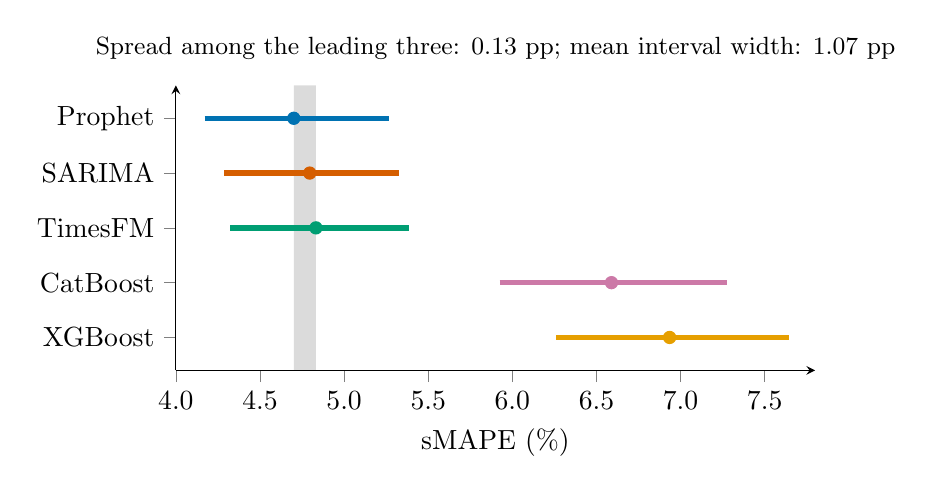
\begin{tikzpicture}
\begin{axis}[
  width=0.80\textwidth, height=5.2cm,
  xlabel={sMAPE (\%)}, xmin=4.0, xmax=7.8,
  xtick={4.0,4.5,5.0,5.5,6.0,6.5,7.0,7.5},
  xticklabel style={/pgf/number format/fixed, /pgf/number format/precision=1,
                     /pgf/number format/zerofill},
  ymin=0.4, ymax=5.6, ytick={5,4,3,2,1}, yticklabels={Prophet,SARIMA,TimesFM,CatBoost,XGBoost},
  axis lines=left, tick align=outside, tick pos=left,
  title style={align=left, font=\small},
  title={Spread among the leading three: 0.13 pp; mean interval width: 1.07 pp},
]
\addplot[draw=none, fill=black, fill opacity=0.14, forget plot]
  coordinates {(4.7010,0.4) (4.8325,0.4) (4.8325,5.6) (4.7010,5.6)}
  \closedcycle;
\addplot[draw=cprophet, line width=2.0pt, mark=none] coordinates {(4.1709,5) (5.2675,5)};
\addplot[only marks, mark=*, mark size=2.2pt, draw=cprophet, fill=cprophet] coordinates {(4.7010,5)};
\addplot[draw=csarima, line width=2.0pt, mark=none] coordinates {(4.2890,4) (5.3270,4)};
\addplot[only marks, mark=*, mark size=2.2pt, draw=csarima, fill=csarima] coordinates {(4.7957,4)};
\addplot[draw=ctimesfm, line width=2.0pt, mark=none] coordinates {(4.3245,3) (5.3851,3)};
\addplot[only marks, mark=*, mark size=2.2pt, draw=ctimesfm, fill=ctimesfm] coordinates {(4.8325,3)};
\addplot[draw=ccatboost, line width=2.0pt, mark=none] coordinates {(5.9248,2) (7.2734,2)};
\addplot[only marks, mark=*, mark size=2.2pt, draw=ccatboost, fill=ccatboost] coordinates {(6.5893,2)};
\addplot[draw=cxgboost, line width=2.0pt, mark=none] coordinates {(6.2614,1) (7.6465,1)};
\addplot[only marks, mark=*, mark size=2.2pt, draw=cxgboost, fill=cxgboost] coordinates {(6.9350,1)};
\end{axis}
\end{tikzpicture}
\caption{sMAPE by model with 95\% block bootstrap intervals over the 103 rolling origin
windows. The grey band spans the point estimates of the three most accurate models.}
\label{fig:smape}
\end{figure}

% gerado por paper_v1b/build_tables.py a partir de paper/tables/tab2_pares.tex -- nao editar a mao
\begin{table}[htbp]
\centering
\small
\caption{Paired differences in sMAPE among the three most accurate models. A positive difference means the first model has the larger error.}
\label{tab:pares}
\begin{tabular}{lrcrc}
\toprule
Comparison & Difference (pp) & 95\% CI & $p$ (bootstrap) & DM cells $p<0.05$ \\
\midrule
Prophet $-$ SARIMA & $-0.095$ & $[-0.367, +0.157]$ & 0.512 & 0 of 6 \\
Prophet $-$ TimesFM & $-0.132$ & $[-0.319, +0.056]$ & 0.171 & 0 of 6 \\
SARIMA $-$ TimesFM & $-0.037$ & $[-0.303, +0.262]$ & 0.768 & 0 of 6 \\
\bottomrule
\end{tabular}

\vspace{0.5em}
\begin{minipage}{\textwidth}
\footnotesize
pp, percentage points. Bootstrap differences are computed within each replicate on the same resampled windows. DM, Diebold-Mariano test with the Harvey-Leybourne-Newbold correction, run separately at each of the six horizons; the column counts horizons with $p<0.05$.
\end{minipage}
\end{table}


The two boosting models were at least 1.76 points behind. All 36 Diebold-Mariano
comparisons of a boosting model with one of the three leading models had $p<0.05$, and the
bootstrap $p$ for each pooled difference was below 0.001.

The seasonal naive method reached 6.27\% (MASE 1.148) and the drift variant 6.18\%. The
three leading models reduced the error of the seasonal naive by about a quarter (MASE 0.860
to 0.887). CatBoost (6.59\%) and XGBoost (6.88\%) did not improve on it. For CatBoost the
paired interval against the seasonal naive was $[-0.056, +0.716]$, and for XGBoost the
interval excluded zero but no Diebold-Mariano cell did, so neither is established as worse
than the reference. The naive method that ignores the annual cycle reached 10.74\%. Most of
what there is to forecast in this series is the annual cycle.

\subsection{Boosting configurations and a tabular foundation model}

No configuration of the tabular models we tried was established as better than the seasonal
naive method (Supplementary Tables~\ref{tab:variantes} and~\ref{tab:optuna}). Rolling window
statistics made both boosting models worse. The changes that helped were those that gave
them the annual cycle: calendar terms and forecasting the seasonal difference
$y_t - y_{t-12}$. The best variant reached 6.09\%, with a paired interval against the
seasonal naive of $[-0.45, +0.10]$. Hyperparameter search restricted to the training period
moved CatBoost from 6.59\% to 6.42\% and XGBoost from 6.88\% to 7.02\%.

TabPFN reached 5.85\%, the best of the tabular models. Its advantage over the seasonal
naive (0.42 points, interval $[-0.698, -0.128]$) was significant only at the one-month
horizon ($p=0.0012$), so it does not meet the criterion over the six-month horizon. It
remained 1.14 points behind Prophet. Because TabPFN was run through a hosted API, its result
is tied to the service version: an earlier client release gave 6.04\%.

\subsection{Removing the pandemic period}

Excluding the COVID-19 windows lowered the error of all three leading models by about the
same amount; Prophet went from 4.70\% to 3.60\% and 3.47\% under the two exclusions, which
remove 27 and 41 of the 103 windows (Supplementary Table~\ref{tab:covid}). No pair among the
three separated in any of the three test periods, and under the wider exclusion SARIMA moved
ahead of Prophet by 0.06 points.

\subsection{Training history}

% gerado por paper_v1b/build_tables.py a partir de paper/tables/tab3_serie.tex -- nao editar a mao
\begin{table}[htbp]
\centering
\small
\caption{sMAPE on the same 36 target months (January 2021 to December 2023) with short and long training history.}
\label{tab:serie}
\begin{tabular}{lrrr}
\toprule
Model & sMAPE, 24--54 months & sMAPE, 132--168 months & Gain (pp) \\
\midrule
Prophet & 7.68 & 5.97 & 1.71 \\
SARIMA & 7.45 & 6.18 & 1.27 \\
TimesFM & 7.30 & 6.07 & 1.23 \\
\bottomrule
\end{tabular}

\vspace{0.5em}
\begin{minipage}{\textwidth}
\footnotesize
The short-history column comes from a run on 2019--2023 data, in which each window had 24 to 54 months of training ($n=186$ forecasts per model); the long-history column is the subset of the main analysis that falls on the same target months ($n=201$). Only the amount of training data differs.
\end{minipage}
\end{table}


On the same 36 target months, the long-history forecasts had 1.23 to 1.71 points lower
sMAPE than the short-history ones (Table~\ref{tab:serie}), about ten times the spread among
the three leading models. With short history, the point ordering was different: TimesFM
first at 7.30\% and Prophet last at 7.68\%, a spread of 0.38 points with a mean interval
width of 2.45 points.

% gerado por paper_v1b/build_tables.py a partir de paper/tables/tab4_janela.tex -- nao editar a mao
\begin{table}[htbp]
\centering
\small
\setlength{\tabcolsep}{4pt}
\caption{sMAPE with an expanding training window and with a window limited to the most recent 60 months, on identical test origins. A negative difference means the expanding window is more accurate.}
\label{tab:janela}
\begin{tabular}{lrrrcrc}
\toprule
Model & Expanding & Sliding 60 & Expanding $-$ Sliding (pp) & 95\% CI & $p$ & DM cells $p<0.05$ \\
\midrule
Prophet & 4.70 & 5.39 & $-0.69$ & $[-1.159, -0.219]$ & 0.005 & 0 of 6 \\
SARIMA & 4.80 & 5.46 & $-0.66$ & $[-1.008, -0.346]$ & 0.000 & 3 of 6 \\
TimesFM & 4.83 & 4.74 & $+0.09$ & $[-0.125, +0.307]$ & 0.424 & 0 of 6 \\
CatBoost & 6.59 & 6.64 & $-0.05$ & $[-0.288, +0.176]$ & 0.661 & 0 of 6 \\
XGBoost & 6.88 & 6.86 & $+0.02$ & $[-0.258, +0.303]$ & 0.879 & 0 of 6 \\
\bottomrule
\end{tabular}

\vspace{0.5em}
\begin{minipage}{\textwidth}
\footnotesize
The expanding window uses 60 to 162 months of training; the sliding window uses the last 60. The bootstrap is paired by window. DM as in Table~\ref{tab:pares}.
\end{minipage}
\end{table}


Limiting training to the most recent 60 months cost SARIMA 0.66 points, meeting the
established criterion, and Prophet 0.69 points, with an interval that excluded zero and no
significant Diebold-Mariano cell (Table~\ref{tab:janela}, Figure~\ref{fig:janela}). TimesFM
did not change ($+0.09$, $p=0.42$). With five years of history, TimesFM had 4.74\% against
5.46\% for SARIMA.

\begin{figure}[htbp]
\centering
% gerado por scripts/build_paper_assets.py -- nao editar a mao
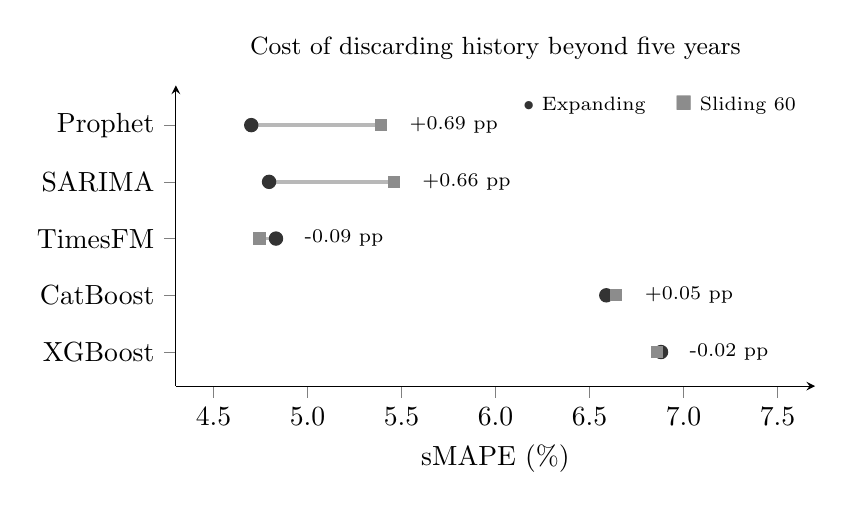
\begin{tikzpicture}
\begin{axis}[
  width=0.80\textwidth, height=5.4cm,
  xlabel={sMAPE (\%)}, xmin=4.3, xmax=7.7,
  xtick={4.5,5.0,5.5,6.0,6.5,7.0,7.5},
  xticklabel style={/pgf/number format/fixed, /pgf/number format/precision=1,
                     /pgf/number format/zerofill},
  ymin=0.4, ymax=5.7, ytick={5,4,3,2,1}, yticklabels={Prophet,SARIMA,TimesFM,CatBoost,XGBoost},
  axis lines=left, tick align=outside, tick pos=left,
  title style={align=left, font=\small},
  title={Cost of discarding history beyond five years},
]
\addplot[draw=black!28, line width=1.2pt, mark=none] coordinates {(4.7010,5) (5.3909,5)};
\addplot[only marks, mark=*, mark size=2.4pt, draw=black!80, fill=black!80] coordinates {(4.7010,5)};
\addplot[only marks, mark=square*, mark size=2.0pt, draw=black!45, fill=black!45] coordinates {(5.3909,5)};
\node[anchor=west, font=\scriptsize, text=black] at (axis cs:5.4909,5) {+0.69 pp};
\addplot[draw=black!28, line width=1.2pt, mark=none] coordinates {(4.7957,4) (5.4588,4)};
\addplot[only marks, mark=*, mark size=2.4pt, draw=black!80, fill=black!80] coordinates {(4.7957,4)};
\addplot[only marks, mark=square*, mark size=2.0pt, draw=black!45, fill=black!45] coordinates {(5.4588,4)};
\node[anchor=west, font=\scriptsize, text=black] at (axis cs:5.5588,4) {+0.66 pp};
\addplot[draw=black!28, line width=1.2pt, mark=none] coordinates {(4.8325,3) (4.7447,3)};
\addplot[only marks, mark=*, mark size=2.4pt, draw=black!80, fill=black!80] coordinates {(4.8325,3)};
\addplot[only marks, mark=square*, mark size=2.0pt, draw=black!45, fill=black!45] coordinates {(4.7447,3)};
\node[anchor=west, font=\scriptsize, text=black] at (axis cs:4.9325,3) {-0.09 pp};
\addplot[draw=black!28, line width=1.2pt, mark=none] coordinates {(6.5893,2) (6.6424,2)};
\addplot[only marks, mark=*, mark size=2.4pt, draw=black!80, fill=black!80] coordinates {(6.5893,2)};
\addplot[only marks, mark=square*, mark size=2.0pt, draw=black!45, fill=black!45] coordinates {(6.6424,2)};
\node[anchor=west, font=\scriptsize, text=black] at (axis cs:6.7424,2) {+0.05 pp};
\addplot[draw=black!28, line width=1.2pt, mark=none] coordinates {(6.8804,1) (6.8569,1)};
\addplot[only marks, mark=*, mark size=2.4pt, draw=black!80, fill=black!80] coordinates {(6.8804,1)};
\addplot[only marks, mark=square*, mark size=2.0pt, draw=black!45, fill=black!45] coordinates {(6.8569,1)};
\node[anchor=west, font=\scriptsize, text=black] at (axis cs:6.9804,1) {-0.02 pp};
\node[anchor=east, font=\scriptsize, text=black] at (axis cs:7.65,5.35)
  {\textcolor{black!80}{$\bullet$} Expanding \quad
    \textcolor{black!45}{$\blacksquare$} Sliding 60};
\end{axis}
\end{tikzpicture}
\caption{sMAPE with an expanding training window and with the last 60 months only, on
identical test origins. The annotation on each row is sliding minus expanding sMAPE, so a
positive value is the accuracy lost by discarding older history.}
\label{fig:janela}
\end{figure}

\subsection{Prediction intervals}

% gerado por paper_v1b/build_tables.py a partir de paper/tables/tab6_calibracao.tex -- nao editar a mao
\begin{table}[htbp]
\centering
\small
\setlength{\tabcolsep}{5pt}
\caption{Empirical coverage and interval score of the nominal 95\% prediction intervals of SARIMA and Prophet, by forecast horizon, over the 103 windows.}
\label{tab:calibracao}
\begin{tabular}{lcccccccr}
\toprule
& \multicolumn{6}{c}{Forecast horizon (months)} & & \\
\cmidrule(lr){2-7}
Model and metric & $h=1$ & $h=2$ & $h=3$ & $h=4$ & $h=5$ & $h=6$ & All & MPIW \\
\midrule
SARIMA, coverage & 0.854 & 0.854 & 0.845 & 0.854 & 0.825 & 0.835 & 0.845 & 1288 \\
Prophet, coverage & 0.796 & 0.786 & 0.796 & 0.767 & 0.738 & 0.748 & 0.772 & 1045 \\
\midrule
SARIMA, interval score & 2792 & 3460 & 3577 & 3532 & 3667 & 3969 & 3500 & --- \\
Prophet, interval score & 4208 & 4342 & 4340 & 4572 & 4640 & 4706 & 4468 & --- \\
\bottomrule
\end{tabular}

\vspace{0.5em}
\begin{minipage}{\textwidth}
\footnotesize
Coverage is the fraction of observed values inside the interval (target 0.950). MPIW, mean interval width in deaths per month. Interval score as in \citet{gneiting2007}: width plus a penalty for each observation outside the interval, proportional to the miss; lower is better.
\end{minipage}
\end{table}


At a nominal 95\%, SARIMA intervals covered 84.5\% of observations and Prophet intervals
77.2\% (Table~\ref{tab:calibracao}). A manager told the outcome would fall inside the
interval nineteen times in twenty would see it fall inside about seventeen times with SARIMA
and fifteen with Prophet. Prophet had the narrower intervals (1{,}045 against 1{,}288 deaths
a month) and the worse interval score (4{,}468 against 3{,}500), and its coverage fell from
0.796 at one month to 0.748 at six; SARIMA stayed between 0.854 and 0.835. The model with
the lowest sMAPE had the worse intervals.

\subsection{Temperature}

% gerado por paper_v1b/build_tables.py a partir de paper/tables/tab5_temperatura.tex -- nao editar a mao
\begin{table}[htbp]
\centering
\small
\setlength{\tabcolsep}{4pt}
\caption{sMAPE with and without monthly minimum temperature as a covariate. TimesFM has no covariate interface in the version used and is not included.}
\label{tab:temperatura}
\begin{tabular}{lrrrcrr}
\toprule
Model & Without & With temp. & Gain (pp) & 95\% CI & DM cells $p<0.05$ & Ceiling \\
\midrule
Prophet & 4.70 & 4.74 & $-0.035$ & $[-0.081, +0.013]$ & 0 of 6 & 4.63 \\
SARIMA & 4.80 & 4.66 & $+0.136$ & $[+0.034, +0.257]$ & 1 of 6 & 4.63 \\
CatBoost & 6.59 & 6.33 & $+0.258$ & $[+0.073, +0.452]$ & 1 of 6 & 6.30 \\
XGBoost & 6.88 & 6.51 & $+0.368$ & $[+0.190, +0.548]$ & 3 of 6 & 6.53 \\
\bottomrule
\end{tabular}

\vspace{0.5em}
\begin{minipage}{\textwidth}
\footnotesize
With temp.: the future covariate is the month-of-year mean of temperature computed from data up to each window's training end, so no future value is used. Ceiling: the observed future temperature, which no real forecast could use; it bounds what a perfect weather forecast could add. Gain is positive when temperature reduces error. DM as in Table~\ref{tab:pares}.
\end{minipage}
\end{table}


Temperature reduced the error of SARIMA (0.136 points), CatBoost (0.258) and XGBoost
(0.368), with intervals excluding zero, and increased the error of Prophet by 0.035 points,
within its interval (Table~\ref{tab:temperatura}). Only XGBoost met the established
criterion, with 3 of 6 significant horizons, and this verdict depended on the computing
environment: on a second machine it had 4 of 6, and with an earlier, unpinned library
version 2 of 6. When calendar terms and seasonal differencing were added to the boosting
models, the gain from temperature fell to 0.076 points for CatBoost and disappeared for
XGBoost ($-0.010$) (Supplementary Table~\ref{tab:tempdiffcal}). Replacing the climatological
covariate with the observed future temperature improved SARIMA by a further 0.03 points.

The series peaks in July, with a mean of 8{,}247 deaths, and reaches its trough in February,
with 6{,}273, an amplitude of 27.2\% around the mean. The seasonal shape was stable over the
fourteen years, including the pandemic period (Figure~\ref{fig:serie}).

\section{Discussion}

On a 14-year monthly series of cardiovascular deaths in S\~ao Paulo state, three models of
different families, a seasonal ARIMA, Prophet and a pre-trained foundation model, could not
be told apart, while nine more years of training history reduced error by about ten times
their spread. The foundation model was the only one that did not lose accuracy when history
was cut to five years. The intervals that two of the models produce covered far less than
their nominal level.

\subsection{Comparison with other studies}

The order of the model families agrees with the large forecasting competitions. In M4, with
100{,}000 series of several frequencies, combinations of statistical methods were among the
most accurate, and none of the six pure machine learning methods beat the combination
benchmark \citep{makridakis2018, makridakis2020}. In M5 most methods, the winner included, were built on LightGBM
\citep{makridakis2022}, but there the task was 42{,}840 related series of Walmart unit sales with calendar and price
information, the setting in which a single model learns across series. Our boosting models had
one series and twelve lags. They improved when given the calendar, through calendar terms,
seasonal differencing or temperature, which in this series acts as a proxy for the month of
the year. The similarity between TimesFM and the classical models also fits evidence that
simple models remain competitive with transformer architectures on standard forecasting
benchmarks \citep{zeng2023}.

Foundation model benchmarks summarise performance across archives of many series
\citep{godahewa2021, aksu2024}. Our result does not contradict them, because a single
series cannot. It shows that the difference between models on one series can be much
smaller than the uncertainty of the comparison, one of the ways in which, as
\citet{hewamalage2023} show, evaluation practice produces spurious conclusions about
forecasting methods. In
our case, the point ordering on the shorter series placed TimesFM first by 0.38 points
inside intervals of 2.45 points, and with more data Prophet had the lowest error. Neither
ordering is informative.

The July peak agrees with the winter excess in myocardial infarction mortality reported for
the city of S\~ao Paulo \citep{sharovsky2002}, and the stability of the seasonal shape over
fourteen years, the pandemic included, is what makes a seasonal model sufficient here. Unlike the long-range projections of \citet{siqueira2020},
our horizon is six months, which is what capacity planning for a winter needs.

\subsection{Interpretation}

Most of the predictable structure of this series is the annual cycle: repeating last year
already gives 6.27\% sMAPE, and the naive method that ignores the cycle gives 10.74\%. Any
model that represents the cycle well reaches about the same accuracy, and the remaining
error is dominated by events no model sees coming, such as the pandemic, which raised the
error of all three leading models alike. This also explains why longer history helps:
more years give a better estimate of the seasonal shape and of the trend, which for
absolute counts includes population growth and ageing.

TimesFM was insensitive to history length because it does not estimate its parameters from
the target series. It brings its prior from pre-training and reads a bounded context. That
is a disadvantage on a long, clean series, where the classical models can learn the same
structure, and an advantage on a short one.

Temperature at monthly resolution added little beyond the calendar: the gain disappeared
once the boosting models had calendar terms, and a perfect future temperature improved
SARIMA by 0.03 points. The cardiovascular effect of cold acts over days \citep{analitis2008,
ferreira2019}, and averaging to monthly minima removes most of that signal. Weekly or daily
series would be needed to test it.

\subsection{Limitations}

We modelled counts, not rates. Part of what the long history adds is therefore population
growth and ageing, and this probably overstates the benefit of long history for
epidemiological change. The series is a single state aggregate, longer and smoother than
any municipal or regional series, which probably makes all models look better than they
would on subunits. We did not stratify by age, sex or cause subgroup, which have different
seasonal patterns. TimesFM was used zero-shot; fine-tuning could change its relative
position. Only two models produced prediction intervals, and both undercovered by 10 to 18
percentage points, so none of the forecasts here can be given to a planner with a
reliable interval. Ill-defined causes were not redistributed; a change in their share
over time would appear in the series as a change in trend.

\subsection{Implications}

For a team forecasting one well-recorded indicator with more than a decade of data, the
choice among SARIMA, Prophet and a foundation model can rest on cost, transparency and
maintenance; SARIMA is the cheapest and had the better intervals. Effort spent extending and
cleaning the historical series is likely to pay more than effort spent on model selection.
A foundation model is a reasonable default where series are short, as for new indicators,
municipalities or strata, though this needs testing on such series. In either case the
intervals should be recalibrated before use; conformal prediction wraps any point forecaster
and offers finite-sample coverage under exchangeability \citep{angelopoulos2023}.

\section{Conclusion}

For monthly cardiovascular mortality in S\~ao Paulo state, the three best models from three
different families were statistically indistinguishable, the length of the training series
mattered about ten times more than the choice among them, and the available prediction
intervals undercovered. The foundation model's advantage appeared only when history was
short.

\section*{Declarations}

\ifdefined\BLIND\else
\textbf{Author contributions (CRediT).} Fabiano Novaes Barcellos Filho: Conceptualization,
Methodology, Software, Formal analysis, Data curation, Writing -- original draft,
Visualization. Isabela Venancio da Silva: Validation, Formal analysis, Investigation,
Writing -- review \& editing, Visualization. Victor Hugo Ovani Marchetti: Investigation,
Validation, Writing -- review \& editing. Alexandre Chiavegatto Filho: Conceptualization,
Resources, Supervision, Writing -- review \& editing.

\textbf{Funding.} This study was financed in part by the Coordena\c{c}\~ao de
Aperfei\c{c}oamento de Pessoal de N\'ivel Superior, Brazil (CAPES), Finance Code 001.
\fi

\textbf{Ethics.} The study used public, de-identified mortality records. Under Resolution
No.~510/2016 of the Brazilian National Health Council, research on publicly accessible
databases without individual identification is exempt from ethics committee review.

\textbf{Competing interests.} The authors declare no competing interests.

\textbf{Data and code availability.} The aggregated monthly series, the temperature series,
all forecasts, uncertainty outputs and the code that produces every table and figure are in
the study repository
\ifdefined\BLIND(address withheld for review)\else
(\url{https://github.com/fabianofilho/cardiovascular-timeseries-prediction})\fi. Individual
records are not redistributed; the extraction script retrieves them from DataSUS.

\textbf{Use of artificial intelligence.} The authors used an AI assistant (Claude,
Anthropic) to write analysis code and to draft and revise the manuscript text. The authors
chose the questions and design, reviewed every analysis and number, and take full
responsibility for the content. The tool is not an author.

\bibliographystyle{unsrtnat}
\bibliography{refs/references}

% Material suplementar, compilado no fim do manuscrito para as referencias cruzadas
% funcionarem. Para a submissao, separar em arquivo proprio.
\clearpage
\appendix
\setcounter{table}{0}
\setcounter{figure}{0}
\setcounter{section}{0}
\renewcommand{\thetable}{S\arabic{table}}
\renewcommand{\thefigure}{S\arabic{figure}}
\renewcommand{\thesection}{S\arabic{section}}

\begin{center}
\large\bfseries Supplementary Material
\end{center}

\section{Computing environment}\label{sec:s-repro}

XGBoost is deterministic within one environment, but its accuracy on this task changed with
the library version and the number of fitting threads. With code, data and seed fixed, sMAPE
ranged from 6.80\% to 6.98\% across seven released versions and five thread counts. CatBoost
did not move by more than a tenth of a basis point under the same variation. We therefore
pinned the XGBoost version and fitted it on one thread; the reported 6.88\% comes from that
environment. On a second machine with a different processor architecture, the same versions
and one thread gave 6.83\% for XGBoost and 6.41\% for its temperature variant (6.51\% in
the pinned environment). This
difference is small against every comparison between models in the paper, but it changes
the count of significant horizons for the temperature gain of XGBoost (main text, Temperature).

Prophet derives its interval bounds from a finite sample of posterior draws, which we seeded
at every window. Without the seed the bounds moved by 34 to 53 deaths between two fits of
the same window. Across machines, 63 of the 103 Prophet point forecasts differed by up to 49
deaths, which left coverage at 0.772 and moved sMAPE from 4.701\% to 4.700\%.

TabPFN was run through a hosted inference API, so its model version is outside the pinned
environment. The same protocol gave 6.04\% with an earlier client release and 5.85\% with
the current one.

\section{Boosting configurations}

% gerado por paper_v1b/build_tables.py a partir de paper/tables/tab7_variantes.tex -- nao editar a mao
\begin{table}[htbp]
\centering
\small
\setlength{\tabcolsep}{4pt}
\caption{Feature engineering variants for the two gradient boosting models, under the protocol of Table~\ref{tab:desempenho}. The last two columns compare each CatBoost variant with the seasonal naive method.}
\label{tab:variantes}
\begin{tabular}{lrrrrcc}
\toprule
& \multicolumn{2}{c}{CatBoost} & \multicolumn{2}{c}{XGBoost}
& \multicolumn{2}{c}{CatBoost vs seasonal naive} \\
\cmidrule(lr){2-3} \cmidrule(lr){4-5} \cmidrule(lr){6-7}
Variant & sMAPE & MASE & sMAPE & MASE & 95\% CI of $\Delta$ & DM \\
\midrule
Lags only (as reported) & 6.59 & 1.213 & 6.88 & 1.263 & $[-0.06, +0.72]$ & 0/6 \\
+ rolling window statistics & 6.79 & 1.248 & 6.95 & 1.275 & $[+0.16, +0.90]$ & 0/6 \\
+ Fourier calendar terms & 6.27 & 1.150 & 6.61 & 1.214 & $[-0.37, +0.39]$ & 0/6 \\
Seasonal differencing & 6.20 & 1.142 & 6.35 & 1.166 & $[-0.37, +0.23]$ & 0/6 \\
Differencing + windows + calendar & 6.14 & 1.129 & 6.44 & 1.181 & $[-0.43, +0.14]$ & 0/6 \\
As above, direct multi-step & 6.09 & 1.126 & 6.39 & 1.183 & $[-0.45, +0.10]$ & 0/6 \\
\midrule
Seasonal naive (benchmark) & \multicolumn{4}{c}{6.27 \quad 1.148} & --- & --- \\
\bottomrule
\end{tabular}

\vspace{0.5em}
\begin{minipage}{\textwidth}
\footnotesize
$\Delta$, CatBoost minus seasonal naive sMAPE, with a paired bootstrap 95\% CI. DM, horizons with $p<0.05$ out of six. Direct multi-step fits one model per horizon.
\end{minipage}
\end{table}


% gerado por paper_v1b/build_tables.py a partir de paper/tables/revisao_tab_optuna.tex -- nao editar a mao
\begin{table}[htbp]
\centering
\small
\setlength{\tabcolsep}{4pt}
\caption{Bayesian hyperparameter search for the two gradient boosting models.}
\label{tab:optuna}
\begin{tabular}{lrrrrrrr}
\toprule
& \multicolumn{3}{c}{sMAPE (\%)} & \multicolumn{2}{c}{Gain (pp)} & & \\
\cmidrule(lr){2-4} \cmidrule(lr){5-6}
Model & Untuned & Training-only & Test-exposed & Training-only & Test-exposed & Trials & Hours \\
\midrule
CatBoost & 6.59 & 6.42 & 6.35 & $+0.17$ & $+0.24$ & 40 + 60 & 2.1 \\
XGBoost & 6.88 & 7.02 & 6.25 & $-0.13$ & $+0.63$ & 40 + 60 & 1.1 \\
\midrule
Seasonal naive & \multicolumn{3}{c}{6.27} & --- & --- & --- & --- \\
\bottomrule
\end{tabular}

\vspace{0.5em}
\begin{minipage}{\textwidth}
\footnotesize
Training-only: 40 trials with the search restricted to the first 60 months, so no test window enters it. Test-exposed: 60 trials allowed to score on the test windows, an upper bound that a real procedure cannot reach. Gain is positive when the search improved on the untuned configuration of Table~\ref{tab:desempenho}.
\end{minipage}
\end{table}


Table~\ref{tab:variantes} changes one element of the boosting feature set at a time. Rolling
window statistics made both models worse. Fourier calendar terms and forecasting the
seasonal difference helped, and the best combination with one model per horizon reached
6.09\% for CatBoost against 6.27\% for the seasonal naive method, with a paired interval
containing zero and no significant horizon. In Table~\ref{tab:optuna}, the search restricted
to the training period improved CatBoost by 0.17 points and made XGBoost 0.13 points worse.
With the test windows exposed, CatBoost reached 6.35\% and XGBoost 6.25\%, 0.02 points ahead
of the seasonal naive method; these values come from configurations selected on the test set
and bound what tuning could achieve.

The best feature engineering variant also lost accuracy under the 60-month sliding window:
0.50 points for CatBoost and 0.41 for XGBoost. Only the aggregate metrics of that run were
kept, so it has no paired interval.

\section{TabPFN}

TabPFN received the same twelve lags as the boosting models. Its sMAPE of 5.85\% was 0.74
points ahead of CatBoost and 1.03 ahead of XGBoost. Against the seasonal naive method its
advantage was 0.42 points (interval $[-0.698, -0.128]$), and against the drift variant 0.33
points ($[-0.622, -0.031]$). The Diebold-Mariano test was significant only at the one-month
horizon ($p=0.0012$ and $p=0.0044$), with $p$ above 0.35 from the third horizon onward, so
the advantage is confined to the first month. SARIMA was ahead of TabPFN in four of six
horizons.

\section{COVID-19 period}

% gerado por paper_v1b/build_tables.py a partir de paper/tables/tab8_covid.tex -- nao editar a mao
\begin{table}[htbp]
\centering
\small
\setlength{\tabcolsep}{5pt}
\caption{sMAPE of the three most accurate models with and without the COVID-19 period in the test set.}
\label{tab:covid}
\begin{tabular}{lrrrrcc}
\toprule
& & \multicolumn{3}{c}{sMAPE (\%)} & \multicolumn{2}{c}{Leading three} \\
\cmidrule(lr){3-5} \cmidrule(lr){6-7}
Test period & Windows & Prophet & SARIMA & TimesFM & Pairs separated & Worst DM \\
\midrule
Full test period & 103 & 4.70 & 4.80 & 4.83 & 0 of 3 & 0 of 6 \\
Excluding 2020-03 to 2021-12 & 76 & 3.60 & 3.74 & 3.66 & 0 of 3 & 0 of 6 \\
Excluding 2020-01 to 2022-12 & 62 & 3.47 & 3.41 & 3.59 & 0 of 3 & 0 of 6 \\
\bottomrule
\end{tabular}

\vspace{0.5em}
\begin{minipage}{\textwidth}
\footnotesize
Windows whose test months overlap the excluded range are dropped whole, so the pairing is kept; no model is refitted. Pairs separated: paired comparisons among the three whose interval excludes zero and whose DM test reaches $p<0.05$ in at least three horizons. Worst DM: the largest count of significant horizons in any pair.
\end{minipage}
\end{table}


\section{Temperature and the calendar}

% gerado por paper_v1b/build_tables.py a partir de paper/tables/revisao_tab_temp_diffcal.tex -- nao editar a mao
\begin{table}[htbp]
\centering
\small
\setlength{\tabcolsep}{5pt}
\caption{Temperature gain for the boosting models with and without explicit calendar terms and seasonal differencing.}
\label{tab:tempdiffcal}
\begin{tabular}{lrrr}
\toprule
Model and feature set & Without temp. & With temp. & Gain (pp) \\
\midrule
CatBoost, lags only & 6.59 & 6.33 & $+0.258$ \\
CatBoost, + calendar and seasonal difference & 6.13 & 6.05 & $+0.076$ \\
\midrule
XGBoost, lags only & 6.88 & 6.51 & $+0.368$ \\
XGBoost, + calendar and seasonal difference & 6.37 & 6.38 & $-0.010$ \\
\bottomrule
\end{tabular}

\vspace{0.5em}
\begin{minipage}{\textwidth}
\footnotesize
Gain in percentage points, positive when temperature reduces error. The lags-only rows reproduce Table~\ref{tab:temperatura}.
\end{minipage}
\end{table}


\begin{figure}[htbp]
\centering
% gerado por scripts/build_paper_assets.py -- nao editar a mao
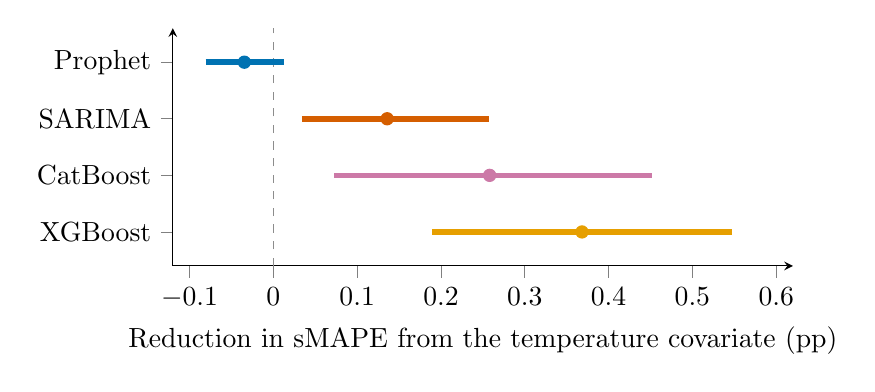
\begin{tikzpicture}
\begin{axis}[
  width=0.78\textwidth, height=4.6cm,
  xlabel={Reduction in sMAPE from the temperature covariate (pp)},
  xmin=-0.12, xmax=0.62,
  % com valores pequenos o pgfplots gera tick automatico em notacao cientifica
  % (-5 \cdot 10^-2) e os rotulos colidem. Tick e formato explicitos.
  xtick={-0.1,0,0.1,0.2,0.3,0.4,0.5,0.6},
  scaled x ticks=false,
  xticklabel style={/pgf/number format/fixed, /pgf/number format/precision=1},
  ymin=0.4, ymax=4.6, ytick={4,3,2,1}, yticklabels={Prophet,SARIMA,CatBoost,XGBoost},
  axis lines=left, tick align=outside, tick pos=left,
]
\draw[black!45, dashed, line width=0.6pt]
  (axis cs:0,0.4) -- (axis cs:0,4.6);
\addplot[draw=cprophet, line width=2.0pt, mark=none] coordinates {(-0.0808,4) (0.0129,4)};
\addplot[only marks, mark=*, mark size=2.2pt, draw=cprophet, fill=cprophet] coordinates {(-0.0346,4)};
\addplot[draw=csarima, line width=2.0pt, mark=none] coordinates {(0.0340,3) (0.2573,3)};
\addplot[only marks, mark=*, mark size=2.2pt, draw=csarima, fill=csarima] coordinates {(0.1358,3)};
\addplot[draw=ccatboost, line width=2.0pt, mark=none] coordinates {(0.0728,2) (0.4519,2)};
\addplot[only marks, mark=*, mark size=2.2pt, draw=ccatboost, fill=ccatboost] coordinates {(0.2581,2)};
\addplot[draw=cxgboost, line width=2.0pt, mark=none] coordinates {(0.1898,1) (0.5476,1)};
\addplot[only marks, mark=*, mark size=2.2pt, draw=cxgboost, fill=cxgboost] coordinates {(0.3683,1)};
\end{axis}
\end{tikzpicture}
\caption{Reduction in sMAPE from adding monthly minimum temperature under the climatology
policy, with 95\% paired bootstrap intervals. Positive values favour the model with
temperature.}
\label{fig:temp}
\end{figure}

\section{Error by horizon and seasonal profile}

\begin{figure}[htbp]
\centering
% gerado por scripts/build_paper_assets.py -- nao editar a mao
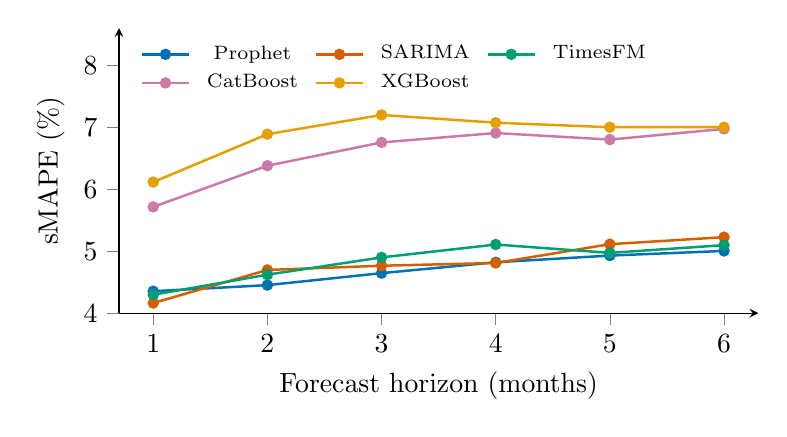
\begin{tikzpicture}
\begin{axis}[
  width=0.80\textwidth, height=5.2cm,
  xlabel={Forecast horizon (months)}, ylabel={sMAPE (\%)},
  xmin=0.7, xmax=6.3, xtick={1,2,3,4,5,6},
  axis lines=left, tick align=outside, tick pos=left,
  legend style={at={(0.02,0.98)}, anchor=north west, draw=none, fill=none,
                 font=\scriptsize, legend columns=3, column sep=4pt},
  ymin=4, ymax=8.6, ytick={4,5,6,7,8},
  % Sem o ymin e o ytick explicitos, a escolha automatica punha a marca mais baixa em
  % 5 e os tres modelos lideres ficavam abaixo dela, sem nenhuma referencia de leitura,
  % com o ponto do SARIMA em h=1 encostado no eixo.
]
\addplot[draw=cprophet, mark=*, mark size=1.6pt, line width=0.9pt, mark options={draw=cprophet, fill=cprophet}] coordinates {(1,4.3538) (2,4.4520) (3,4.6456) (4,4.8209) (5,4.9294) (6,5.0041)};
\addplot[draw=csarima, mark=*, mark size=1.6pt, line width=0.9pt, mark options={draw=csarima, fill=csarima}] coordinates {(1,4.1625) (2,4.6971) (3,4.7652) (4,4.8096) (5,5.1129) (6,5.2266)};
\addplot[draw=ctimesfm, mark=*, mark size=1.6pt, line width=0.9pt, mark options={draw=ctimesfm, fill=ctimesfm}] coordinates {(1,4.2967) (2,4.6208) (3,4.8998) (4,5.1074) (5,4.9729) (6,5.0975)};
\addplot[draw=ccatboost, mark=*, mark size=1.6pt, line width=0.9pt, mark options={draw=ccatboost, fill=ccatboost}] coordinates {(1,5.7154) (2,6.3801) (3,6.7560) (4,6.9079) (5,6.8022) (6,6.9744)};
\addplot[draw=cxgboost, mark=*, mark size=1.6pt, line width=0.9pt, mark options={draw=cxgboost, fill=cxgboost}] coordinates {(1,6.1161) (2,6.8891) (3,7.1997) (4,7.0746) (5,7.0017) (6,7.0013)};
\legend{Prophet,SARIMA,TimesFM,CatBoost,XGBoost}
\end{axis}
\end{tikzpicture}
\caption{sMAPE by forecast horizon, $n=103$ windows per cell.}
\label{fig:horizonte}
\end{figure}

\begin{figure}[htbp]
\centering
% gerado por scripts/build_paper_assets.py -- nao editar a mao
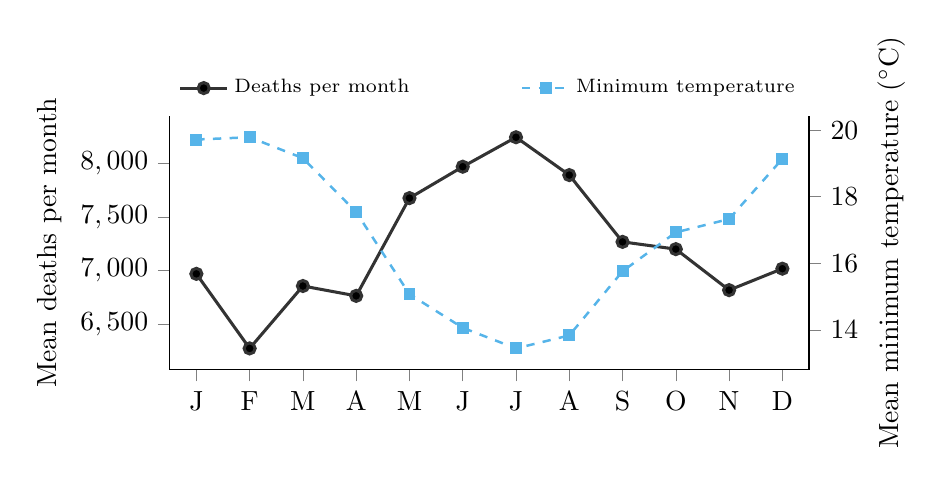
\begin{tikzpicture}
\begin{axis}[
  width=0.80\textwidth, height=4.8cm,
  axis y line*=left, axis x line*=bottom,
  xmin=0.5, xmax=12.5, xtick={1,...,12}, xticklabels={J,F,M,A,M,J,J,A,S,O,N,D},
  ylabel={Mean deaths per month}, ylabel style={text=black},
  scaled y ticks=false, ytick={6500,7000,7500,8000},
  yticklabel style={text=black, /pgf/number format/fixed,
                     /pgf/number format/1000 sep={,}},
  tick align=outside,
  legend style={at={(0,1.03)}, anchor=south west, draw=none, fill=none,
                 font=\scriptsize, text=black},
]
\addplot[draw=black!80, mark=*, mark size=2.0pt, line width=1.1pt]
  coordinates {(1,6969.9) (2,6272.8) (3,6856.3) (4,6764.0) (5,7678.1) (6,7971.6) (7,8247.2) (8,7893.4) (9,7268.9) (10,7201.0) (11,6817.7) (12,7018.1)};
\addlegendentry{Deaths per month}
\end{axis}
\begin{axis}[
  width=0.80\textwidth, height=4.8cm,
  axis y line*=right, axis x line=none,
  xmin=0.5, xmax=12.5,
  ylabel={Mean minimum temperature ($^\circ$C)}, ylabel style={text=black},
  yticklabel style={text=black},
  tick align=outside,
  legend style={at={(1,1.03)}, anchor=south east, draw=none, fill=none,
                 font=\scriptsize, text=black},
]
\addplot[draw=ctemp, mark=square*, mark size=1.7pt, line width=0.9pt, dashed,
         mark options={draw=ctemp, fill=ctemp, solid}]
  coordinates {(1,19.72) (2,19.79) (3,19.16) (4,17.54) (5,15.07) (6,14.06) (7,13.44) (8,13.83) (9,15.76) (10,16.93) (11,17.33) (12,19.14)};
\addlegendentry{Minimum temperature}
\end{axis}
\end{tikzpicture}
\caption{Mean cardiovascular deaths by month of year (left axis) and mean monthly minimum
temperature at station A701 (right axis), 2010--2023.}
\label{fig:sazonal}
\end{figure}


\end{document}
